\documentclass[10pt,a4paper]{article}


\usepackage[utf8]{inputenc}
\usepackage[spanish,english, es-tabla, es-noshorthands]{babel}


\usepackage{siunitx}
\usepackage{amsmath}
\usepackage{amsfonts}
\usepackage{amssymb}
\usepackage{float}
\usepackage{textcomp}
\usepackage{siunitx}
\usepackage{graphicx, wrapfig}
\usepackage{caption}
\usepackage{subfig}
%\usepackage{subcaption}
\usepackage{multicol}
\usepackage{multirow}

\title{PLL}


\begin{document}
\section{PLL: Phase Locked Loop}

\subsection{Introducción}

Un lazo de seguimiento de fase, o phase locked loop, es un sistema de control que genera una señal en su salida cuya fase está relacionada con la fase de la señal en su entrada. En el presente informe, se implementa un PLL mediante el uso de un circuito integrado de bajo consumo, el CD4046B, que consta de un oscilador controlado por voltaje (VCO, por sus siglas en inglés), dos comparadores de fase y un filtro pasa-bajos. Se buscara saber acerca de su funcionamiento y cuales sus limites mientras opera. 
Se preparó el CD4046 con un setup recomendado por la cátedra que se muestra en la figura \ref{fig:Circuito PLL}. Teniendo en cuenta que no se puede colocar una señal negativa en la entrada se procedió a trabajar sobre el circuito armado.

\begin{figure}[H]
	\centering
	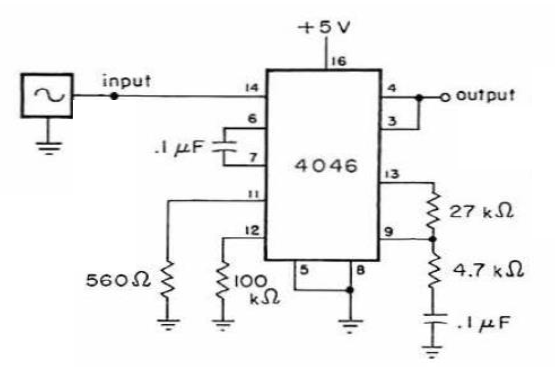
\includegraphics[width= 0.8\textwidth]{../1. PLL/Imagenes/Circuito PLL.png} 
	\label{fig:Circuito PLL}
	\caption{Setup recomendado}
\end{figure}

\subsection{Funcionamiento de un PLL}

Lo que se muestra en la Figura \ref{DiagramaBloquePLL} es un diagrama de bloques de un PLL básico. Se asume que hay una señal de entrada que al ingresar, se la multiplica en un comparador de fase por la salida de un VCO cuya frecuencia, seleccionada en el diseño, es de $f_0$. El producto de la multiplicación es filtrado por un filtro pasa-bajos(LPF) de forma tal que se elimina el ripple y el ruido de alta frecuencia, solo quedando en la salida una tensión proporcional a la diferencia de fase instantánea (la integral de la diferencia de frecuencia) entre las señales multiplicadas. Esta tensión controla la frecuencia del VCO. Si no hay señal en la entrada, no hay voltaje de error a la salida del comparador, por lo que tampoco lo hay a la salida del LPF. En esta situación, el VCO está fijo en su frecuencia central, $f_0$.


\begin{figure}[H]
	\centering
	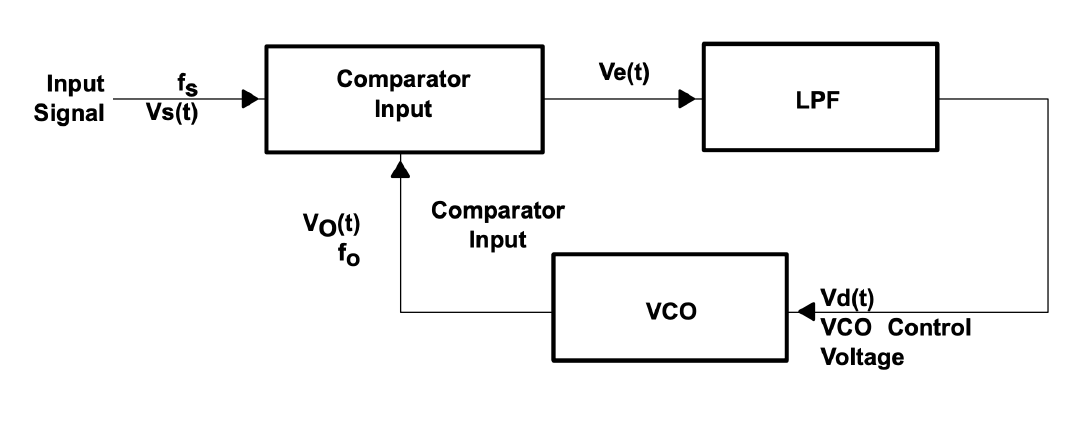
\includegraphics[width=1\textwidth]{../1. PLL/Imagenes/Diagrama bloque PLL.png}
	\caption{Diadrama de bloque de un PLL}
	\label{DiagramaBloquePLL}
\end{figure}

La entrada al VCO varía reduciendo la diferencia de frecuencia entre el VCO y la señal de entrada y a su vez es proporcional a esta diferencia, logrando que la frecuencia del VCO tienda a la frecuencia de la señal de entrada, en otras palabras, realiza un seguimiento de la misma. Cuando se llega a esta condición se dice que el sistema está \textit{"amarrado"}.

\subsubsection{Rango de enganche}

Utilizando un comparador de fase cuya salida es proporcional al seno del ángulo de error de fase, la tensión de error ve, tras pasar por el filtro pasa-bajos, será:

\begin{equation}
	v_e(t) = K_1 f(t)*sin[\phi_i(t)-\phi_o(t)]
	\label{EqVe}
\end{equation}

siendo: 

\begin{equation}
	K_1 = \frac{A_{in}.A_{VCO}}{2}
\end{equation}

Donde $A_{in}$ es la amplitud de la señal de entrada y $A_{VCO}$ es la amplitud de la salida del VCO. $K_1$ representa aquí la ganancia de conversión del comparador de fase, y $f(t)$ es la respuesta al impulso del filtro pasa-bajos. Asumiendo que la frecuencia del VCO es una función lineal de la tensión de error, esta será:

\begin{equation}
	\omega_0 = \omega_c + \frac{d\phi_o}{dt}
\end{equation}

Reemplazando $\frac{d\phi_o}{dt}$ por $K_2.v_e(t)$, donde $K_2$ es la sensibilidadde tensión del VCO(con unidades $\frac{rad}{V.s}$), y reemplazando $v_e$ por \ref{EqVe} se obtiene:

\begin{equation}
	\frac{d\phi_i(t)}{dt} = \frac{d\phi}{dt} +K.f(t)*sin\phi(t)
	\label{eq:DerPhi}
\end{equation}

Donde $K = K_1 K_2 [\frac{rad}{s}]$ y $\frac{d\phi_i(t)}{dt}$ representa la diferencia entre la frecuencia de la señal de entrada y la frecuencia de la portadora, $\Delta\omega_i$. Por lo tanto asumiendo que la ganancia del filtro es 1, la solución de la ecuación \ref{eq:DerPhi} para estado estacionario es:

\begin{equation}
	sin(\phi) = \frac{\Delta\omega_i}{K}
	\label{eq:SinPhi}
\end{equation}

De esta última se deduce que el sistema mantiene el enganche de frecuencias siempre que:

\begin{equation}
	|\Delta\omega_i|< K
	\label{eq:DeltaOmega}
\end{equation}

Esta última ecuación \ref{eq:DeltaOmega} determina el rango del enganche.

\subsubsection{Rango de captura}
El rango de captura es el rango de frecuencias dentro del cual la frecuencia del VCO puede sincronizarse con la
frecuencia de la señal de entrada, partiendo de una situación de asincronismo. Si se tiene un filtro ideal que filtra solo las componentes de alta frecuencia y no atenúa las componentes de baja frecuencia de la señal, los rangos de captura y enganche coinciden. Cuando el filtro no es ideal y se quiere acotar el rango de enganche, reduciendo el ancho de banda del sistema, es muy probable que se vea restringido el rango de captura. Esto es un problema, ya que se dificulta el enganche fuera de condiciones iniciales. Con un rango de captura reducido, si se perturba el circuito y se produce un desenganche, no necesariamente se alcanzará nuevamente el sincronismo aunque la frecuencia de entrada se encuentre dentro del rango de enganche.
Si el sistema se encuentra enganchado la transferencia del lazo no se ve afectada por el circuito LPF. Sino que la transfrencia se ve determinada por K, que define el rango del enganche. Sin embargo cuando el sistema no está enganchado, las frecuencias de las señales de entrada del comparador no son las mismas y el VCO se ve controlado por una tensión de error variable, que puede ser atenuada por el LPF. Esto es equivalente a modificar la ganancia del lazo, y es así como se genera la diferencia entre rango de captura y de enganche. Si expresamos la transferencia del LPF como:

\begin{equation}
F(j\omega) = F_{\omega}e^{j\psi(\omega)}
\end{equation}

Se obtiene que la tensión de error es:

\begin{equation}
v_e(t) = K_1F_{\Delta\omega_i}sin(\Delta\omega_i t)
\end{equation}

El valor pico de la tensión para la frecuencia de captura $\omega_{ic}$ es:

\begin{equation}
	\hat{v_{ec}} = K_1F_{\Delta\omega_{ic}}
	\label{eq:VecPico}
\end{equation}

Por definición al alcanzar la frecuencia de captura el circuito entra en estado estacionario. La tensión de error por estado estacionario es:

\begin{equation}
	V_{ec} = K_1 sin\psi_c
	\label{eq:Vec}
\end{equation}

Igualamos las ecuaciones \ref{eq:VecPico} y \ref{eq:Vec} y reemplazamos en la expresión \ref{eq:DerPhi}, obtuvimos que:

\begin{equation}
	v_{ec} = K_1 \frac{\Delta\omega_i}{K}
	\label{eq:finalVec}
\end{equation}

De esta última expresión se deduce que el rango de captura es $(\omega_i-\omega_c , \omega_i+\omega_c)$, siendo $\omega_c = KF_{\Delta\omega_{ic}}$

\subsubsection{Filtros}

El filtro colocado entre la salida del comparador de fase y la entrada del VCO se puede analizar desde diversas perspectivas para entender su necesidad y función.
En primer lugar, se lo puede ver como un adaptador de la salida del comparador. Dependiendo de la implementación del comparador de fase, se pueden dar dos situaciones, y para ambas un filtro pasa-bajos adecuado es la solución.
Puede ocurrir que la salida del comparador tenga dos frecuencias, $\omega_o - \omega_i$ y $\omega_o + \omega_i$ , de modo que el filtro no deja pasar a la frecuencia más alta. Para ello, la frecuencia principal del filtro debe ser tal que elimine a la mayor frecuencia sin afectar a la menor. Aquí se ve que la frecuencia de corte del filtro, de ser muy pequeña, limita los rangos de captura y de amarre.
Otra posibilidad es que la salida del comparador solo tenga como frecuencia , y el pasa-bajos sea necesario para actuar como promediador, ya que un pasa-bajos puede actuar como integrador, utilizando la relación:

\begin{equation}
	<X> = \frac{1}{T} \int_0^T x(t)dt
\end{equation}

Por otra parte, el filtro es utilizado para evitar que por la presencia de ruido a la entrada del circuito el VCO cambie su frecuencia de oscilación, para lo cual se busca que su frecuencia de corte sea baja. En cuanto a la implementación del filtro, se puede colocar cualquier filtro de tipo pasa-bajos, se analizan los filtros RC y RRC.
Para el tipo de filtro RC la transferencia viene dada por:

\begin{equation}
	F(s)= \frac{1}{1+s\tau_p}
\end{equation}

Donde $\tau_p=R1.C$ como se muestra en la siguiente figura:

\begin{figure}[hbtp]
	\centering
	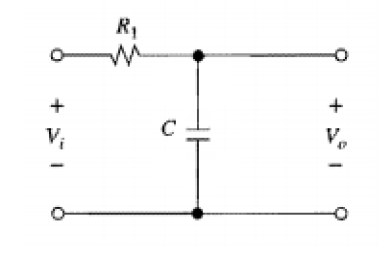
\includegraphics[scale=1]{../1. PLL/Imagenes/Filtro RC.png}
	\caption{Filtro pasa-bajos RC}
	\label{fig:FiltroRC}
\end{figure}

Por lo tanto la transferencia para todo el circuito está dada por:

\begin{equation}
	H(s)= \frac{K/\tau_p}{s^2+ s/\tau_p + K/\tau_p}
	\label{eq:HRC}
\end{equation}

Los parámetros del sistema sub-amortiguado se obtienen de la transferencia y vienen dados por:

\begin{equation}
	\omega_n = \sqrt{K}{\tau_p}
	\label{eq:omeganRC}
\end{equation}

\begin{equation}
	Q = \sqrt{\tau_p K}
	\label{eq:QRC}
\end{equation}

Por otro lado, para el filtro RRC que se muestra en la figura \ref{fig:RRC} se obtiene una transferencia distinta:

\begin{figure}[hbtp]
	\centering
	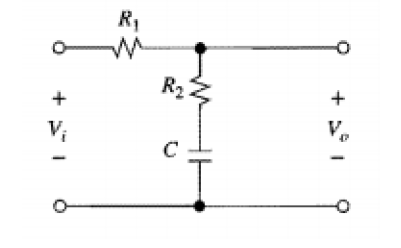
\includegraphics[scale=1]{../1. PLL/Imagenes/Filtro RRC.png}
	\caption{Filtro pasa-bajos RRC}
	\label{fig:RRC}
\end{figure}

\begin{equation}
	F(s)= \frac{1 + s \tau_z}{1 + s\tau_p}
	\label{eq:FRRC}
\end{equation}

Donde $\tau_p=(R1+R2)C $ y $\tau_z=R2C$. Si asumimos $R1<<R2$ se aproxima que $\tau_p \approx R2C$. Viendo todo el sistema del PLL se llega a la siguiente transferencia: 

\begin{equation}
	H(s) = \frac{K(s\tau_z +1)(\tau_z+\tau_p) }{ s^2 + s(1+K\tau_z)/\tau_p + K/\tau_p }
	\label{eq:TransRRC}
\end{equation}

Los parámetros del sistema sub-amortiguado se obtienen de la transferencia y vienen dados por:

\begin{equation}
	\omega_n = \sqrt[K]{\tau_p}
	\label{eq:omeganRRC}
\end{equation}

\begin{equation}
	Q = \frac{ \sqrt{K\tau_p} }{ 1 + \tau_z K }
	\label{eq:QRRC}
\end{equation}

En este caso se puede ver que agregando $R2$ se obtiene independencia entre los valores de $Q$ y $\omega_n$ ya que puedo cambiar $Q$, eligiendo un $\tau_z$ conveniente, sin alterar $\omega_n$.

\subsection{Medición de $K_{VCO}$}
Se nos pidió encontrar la transferencia del VCO de forma práctica, para ello se hicieron mediciones del PLL ya enganchado (con los valores estipulados por la cátedra)  y se calculo tanto la variación en la amplitud como en fase. En la figura \ref{fig:KVCO} se midieron los datos necesarios obteniendo que la variación de amplitud es de $|H(1KHz)|=0,59dB$ y en fase es de $1,44^o$.


\begin{figure}[H]
	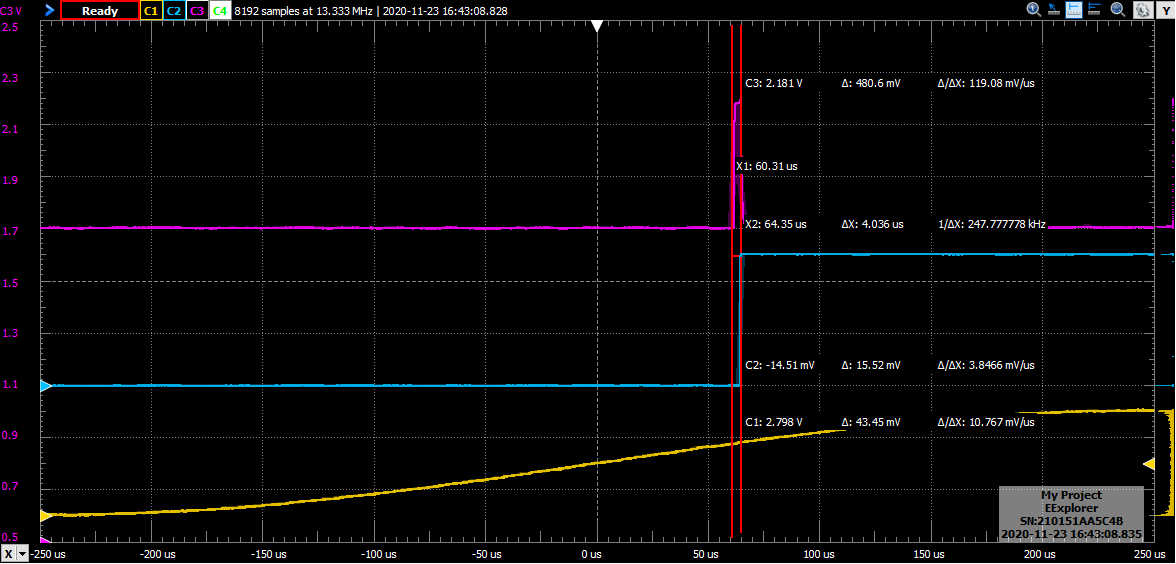
\includegraphics[width= 0.8\textwidth]{../1. PLL/Imagenes/KVCO.png}
	\centering
	\caption{Medición de entrada y salida del VCO}
	\label{fig:KVCO}
\end{figure}

Siendo la señal azul la salida del VCO y la púrpura la entrada.
\newpage

\subsection{Medición de rango de enganche y captura}

A partir de la configuración propuesta por la cátedra se fue variando la frecuencia de la señal de entrada buscando valores donde el enganche se pierde y cuando se recupera, obteniendo así que el rango de enganche se produce entre los $160Hz$ y $2070Hz$. Mientras que el rango de captura es cuando la señal engancha y aunque haya un pequeño cambio o error en la frecuencia no pierde el enganche, esto pasa entre los $160Hz$ y $2050Hz$. Cabe destacar que el valor mínimo de ambos es el mismo, ya que no presenta un cambio destacable entre ambas mediciones, mientras que en el valor máximo del enganche se ve que puede perder el enganche con una pequeña alteración mientras que por debajo del límite de captura estas variaciones no hacen perder el enganche de la señal.
En las siguientes imágenes se puede ver el rango de captura de las señales.

\begin{figure}[H]
	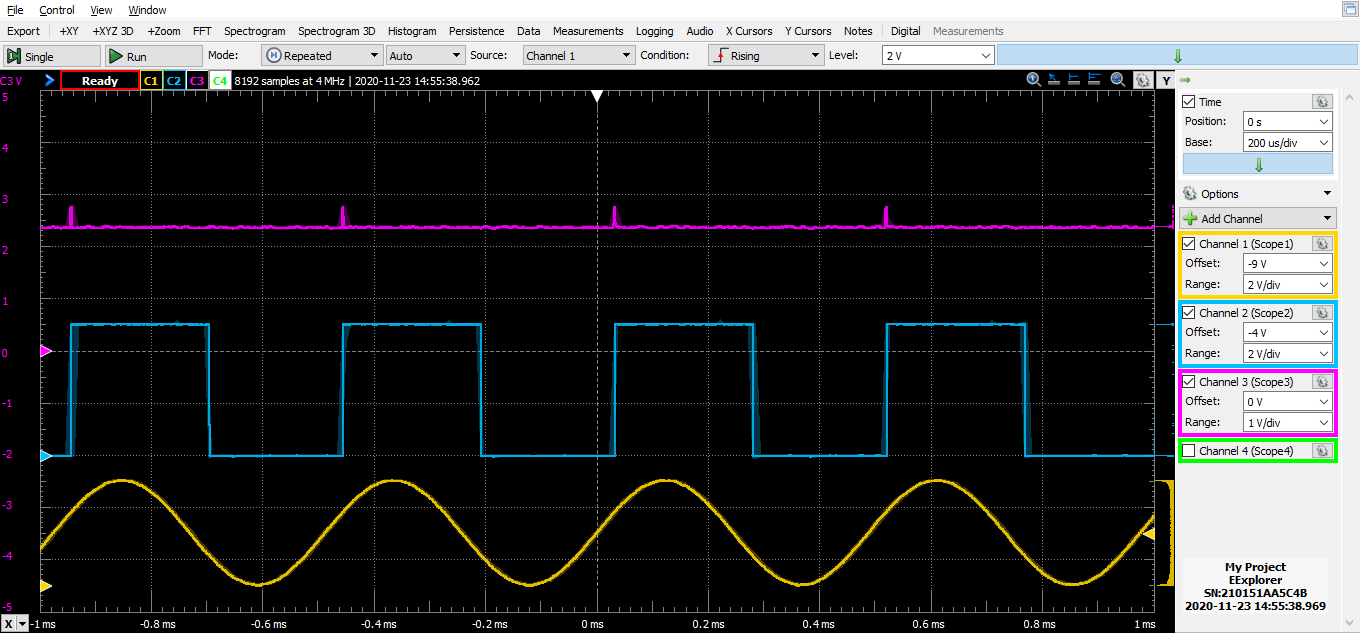
\includegraphics[width= 0.8\textwidth]{../1. PLL/Imagenes/CapturaMax.png}
	\centering
	\caption{Valor de captura máxima ($f_0=2050Hz$)}
	\label{fig:CapMax}
\end{figure}

\begin{figure}[H]
	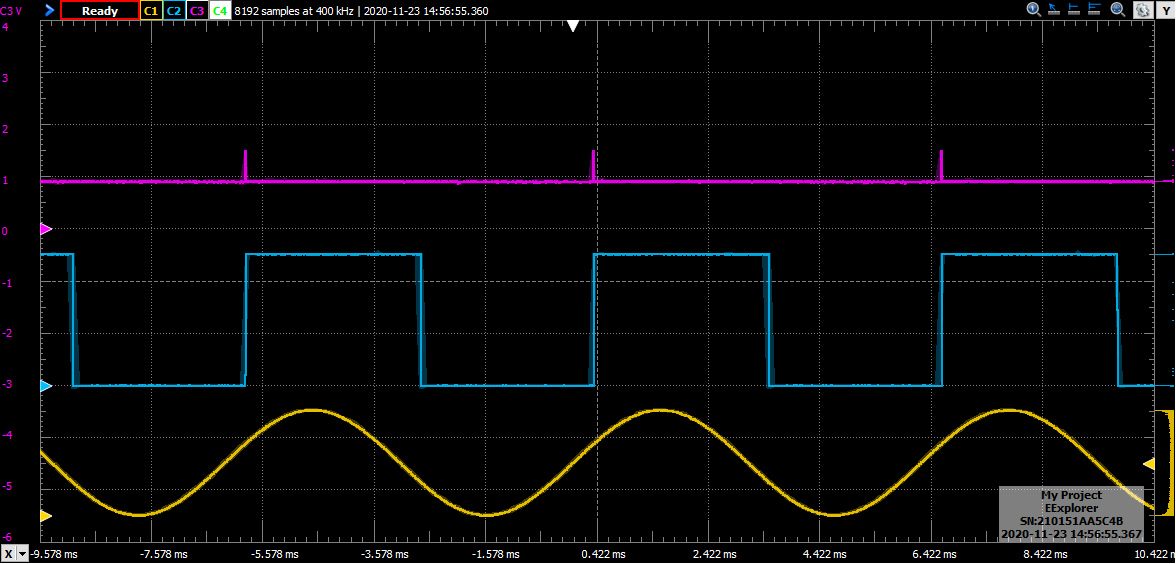
\includegraphics[width= 0.8\textwidth]{../1. PLL/Imagenes/CapturaMin.png}
	\centering
	\caption{Valor de captura mínima ($f_0=160Hz$)}
	\label{fig:CapMin}
\end{figure}

A continuación se pueden ver las mediciones del rango de enganche.

\begin{figure}[H]
	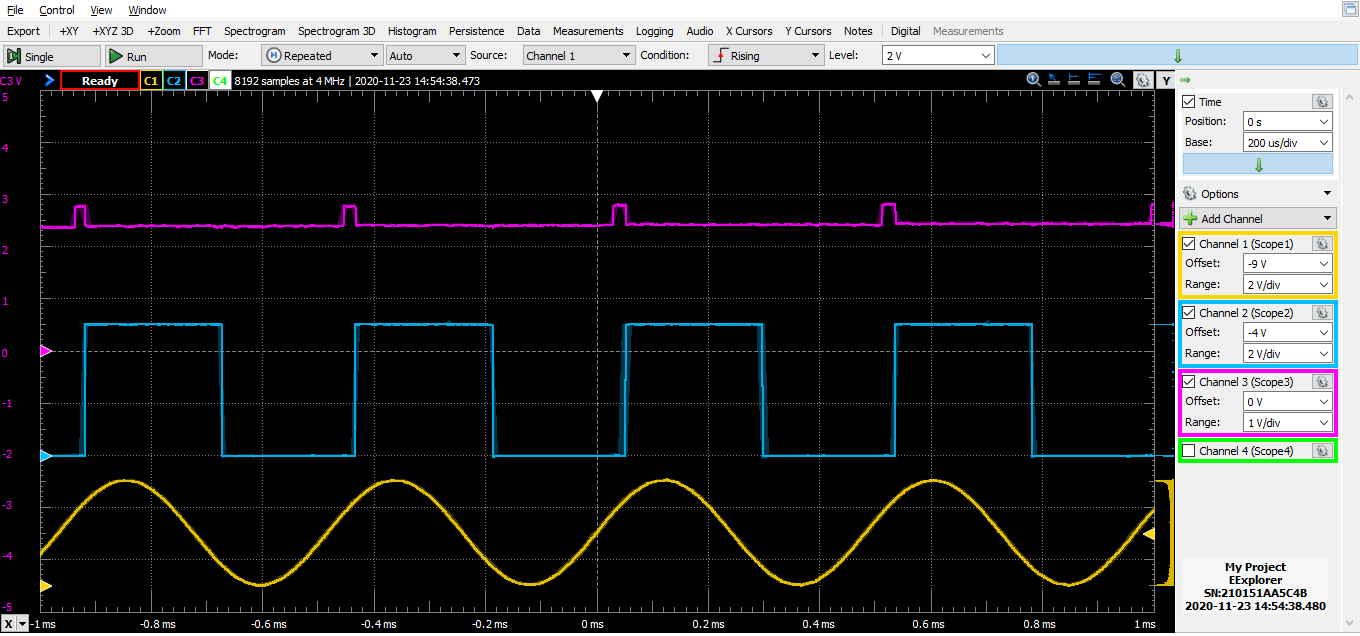
\includegraphics[width= 0.8\textwidth]{../1. PLL/Imagenes/EngancheMax.png}
	\centering
	\caption{Valor de enganche máximo ($f_0=2070Hz$)}
	\label{fig:EngancheMax}
\end{figure}

\begin{figure}[H]
	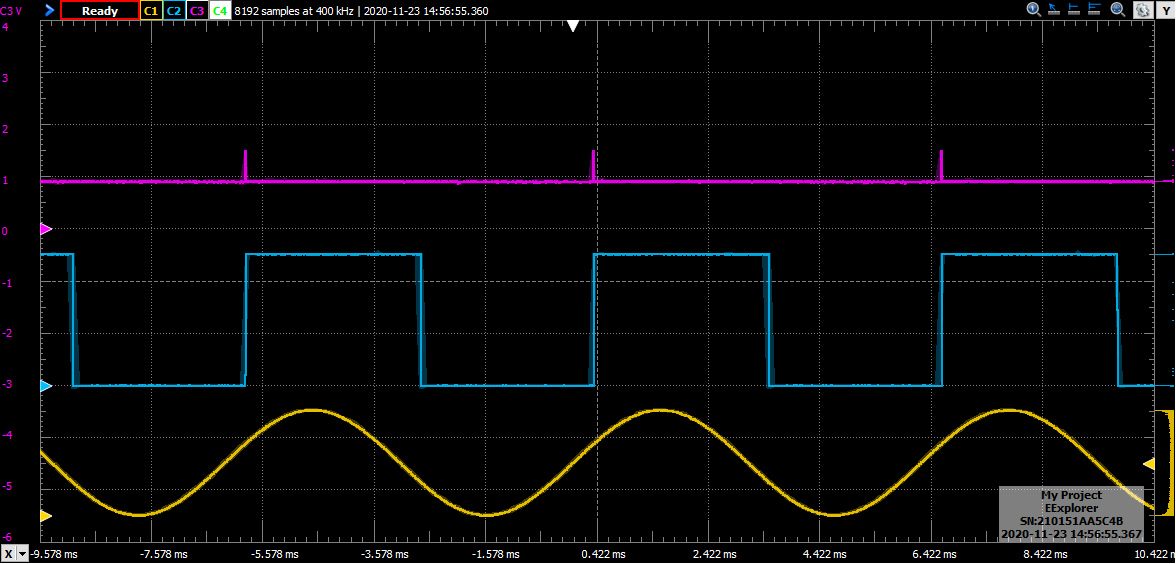
\includegraphics[width= 0.8\textwidth]{../1. PLL/Imagenes/CapturaMin.png}
	\centering
	\caption{Valor de captura mínimo ($f_0=160Hz$)}
	\label{fig:EngancheMin}
\end{figure}

Se debe recordar que estos valores fueron buscados en el equipo de forma manual, ya que se presentaba muy poca diferencia entre que frecuencias variaban los límites de ambos rangos, notándose así que el valor mínimo de ambos llegaron a ser idénticos. 

\subsection{Demodulación en FM}

Una aplicación del PLL es como demodulador de una señal modulada en frecuencia (FM). En este tipo de de modulación se transmiten una señal de interés, la moduladora, a través de una señal portadora de frecuencia mucho mayor. Esto se utiliza dado que la señal de interés, de baja frecuencia, tiene mucho menor alcance que la portadora de alta frecuencia. En la modulación FM, se debe determinar además la máxima variación de frecuencia $\Delta f$ que se le permite a la señal portadora.
Para poder demodular con el EE Digilent, se uso dentro de la opción \textit{Wavegen} la opción de \textit{Modulation} pudiendo elegir tal como se pidió en la consigna una señal de carrier sinusoidal de $1KHz$ con una señal a modular también sinusoidal pero de $200Hz$. En la siguiente imagen se muestra la configuración usada:

\begin{figure}[H]
	\centering
	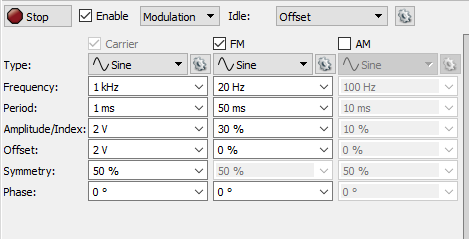
\includegraphics[width= 0.8\textwidth]{../1. PLL/Imagenes/Config Modulacion.png}
	\caption{Configuración para modular del EE Digilent}
	\label{fig:Config Mod}
\end{figure}

A partir de la configuración anterior se fue variando los parámetros de modulación para poder ver los limites que esta tiene, ya que no es posible modular con cualquier señal. A continuación se puede ver la medición pedida, siendo la señal amarilla la señal de entrada, la azul la salida del VCO, la púrpura la entrada del VCO y la verde lo que ve el capacitor del filtro. 

\begin{figure}[H]
	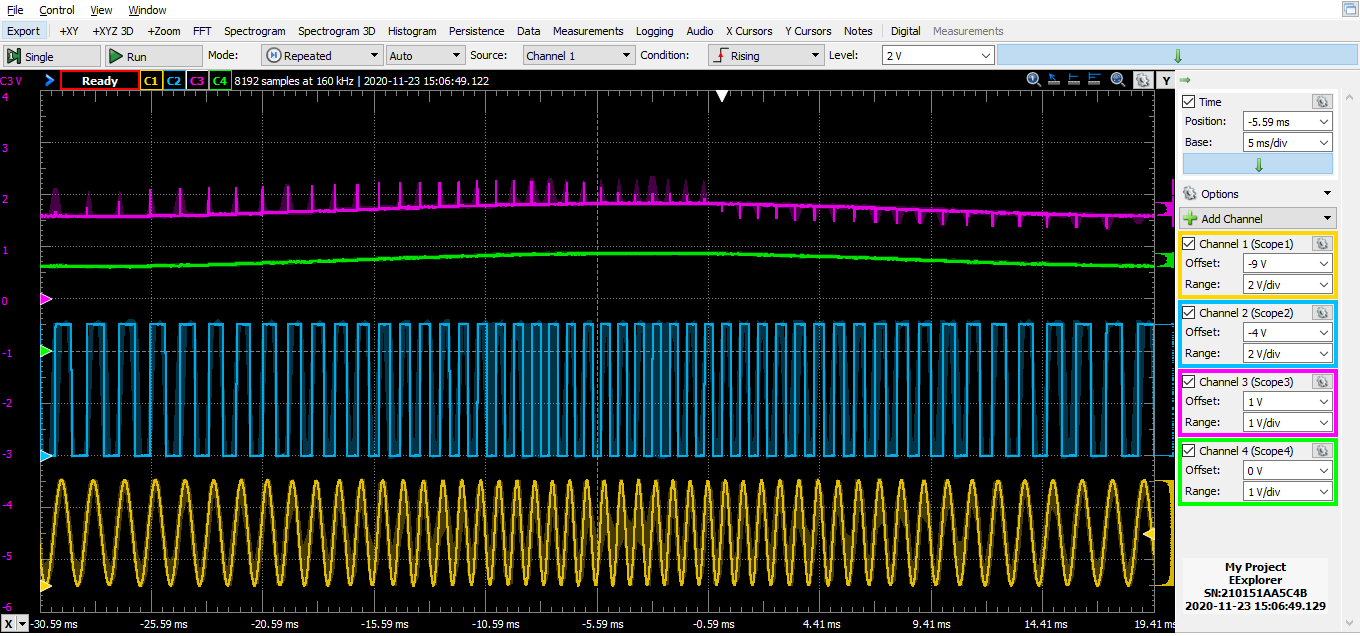
\includegraphics[width= 0.8\textwidth]{../1. PLL/Imagenes/Modulacion030.png}
	\centering
	\caption{Modulación con un índice de $30\%$}
	\label{fig:Mod030}
\end{figure}


En las siguientes mediciones se optó por mostrar solo la señal verde y no púrpura (por los pequeños picos que el capacitor no alcanza a filtrar).
Variando los parámetros se pudo notar que una señal con menos de 3V en la entrada no logra que el PLL lo detecte por lo que no modula la señal. Con un índice del $30\%$ a penas se puede notar la modulación, mientras que con $10\%$ es casi imperceptible la modulación. A partir de un índice de $40\%$ se empieza a notar la modulación.

\begin{figure}[H]
	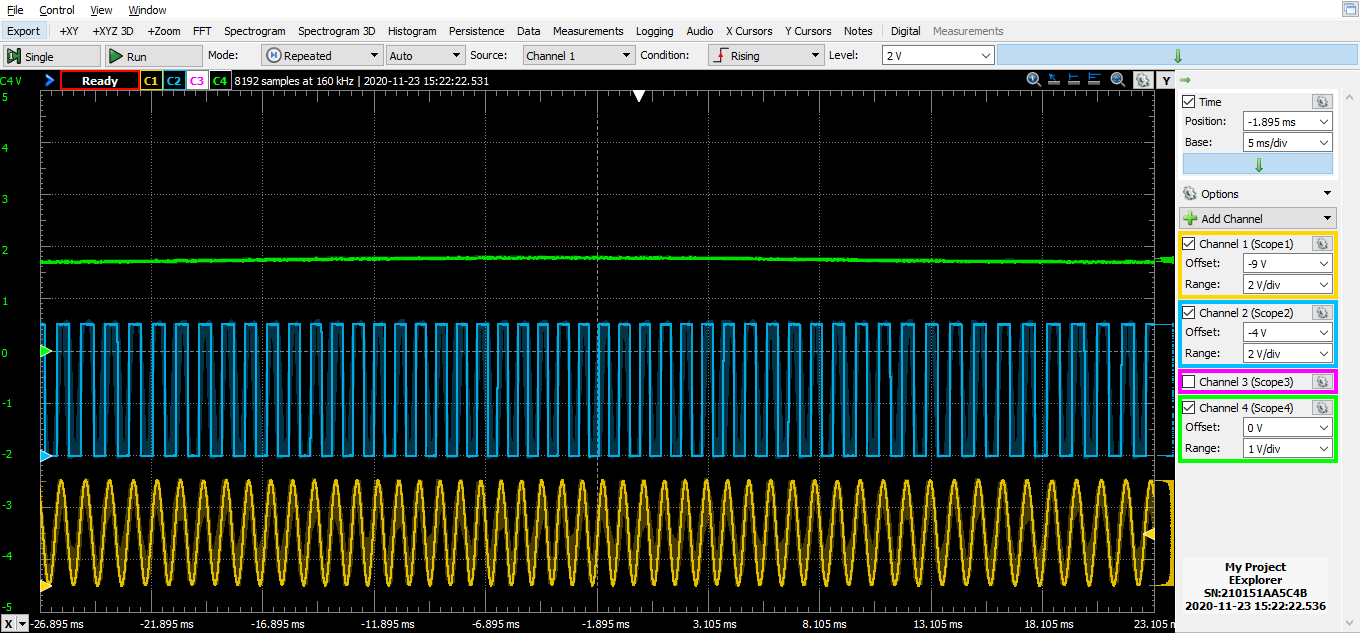
\includegraphics[width= 0.8\textwidth]{../1. PLL/Imagenes/Modulacion010.png}
	\centering
	\caption{Modulación con un índice de $10\%$}
\end{figure}

\begin{figure}[H]
	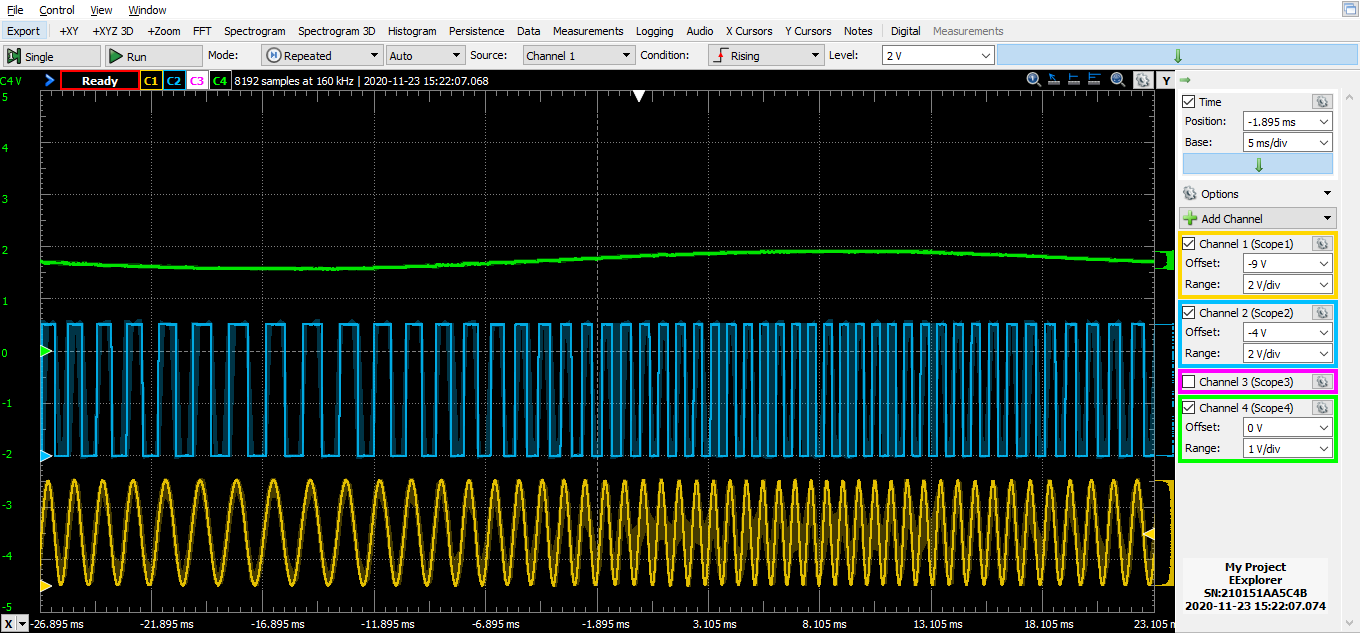
\includegraphics[width= 0.8\textwidth]{../1. PLL/Imagenes/Modulacion040.png}
	\centering
	\caption{Modulación con un índice de $40\%$}
\end{figure}

Con un índice de $\Delta f_c/f_c =80\%$ la modulación pierde forma haciendo que la medición empiece mostrar pequeños errores en la modulación(señal verde), mientras que con un índice del $90\%$ se puede percibir que la modulación no se esta llevando a cabo ya que la señal que se espera pierde su forma.


\begin{figure}[H]
	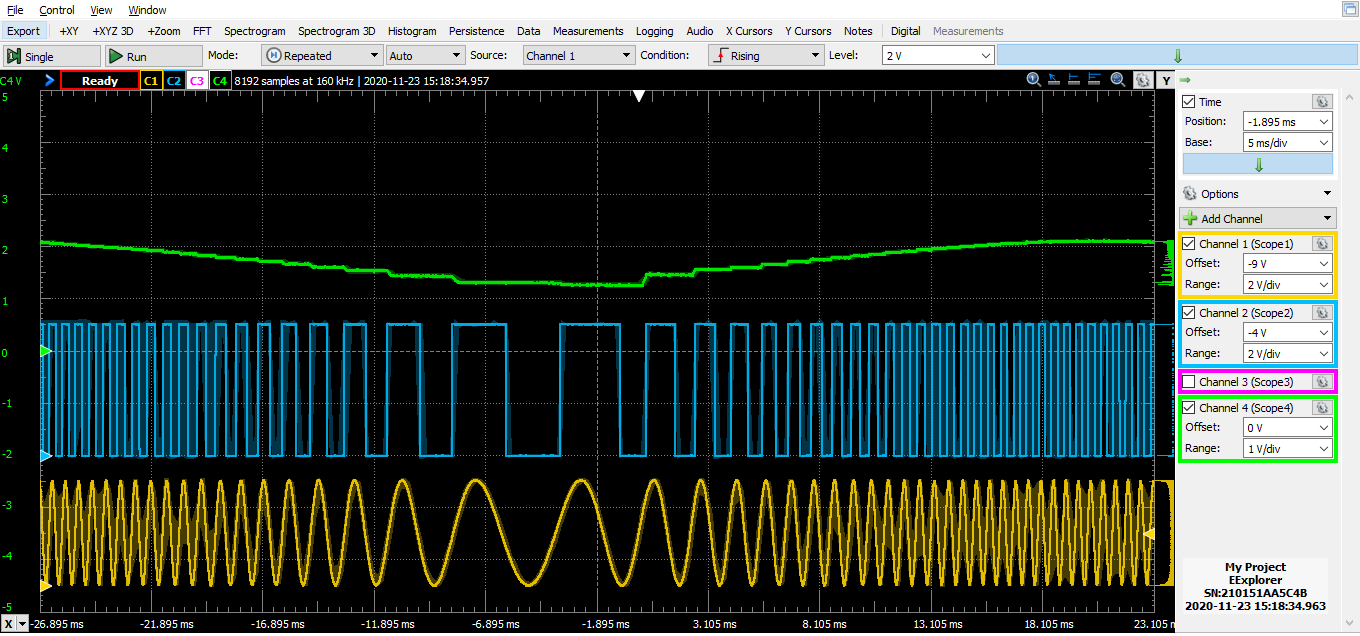
\includegraphics[width= 0.8\textwidth]{../1. PLL/Imagenes/Modulacion080.png}
	\centering
	\caption{Modulación con un índice de $80\%$}
\end{figure}

\begin{figure}[H]
	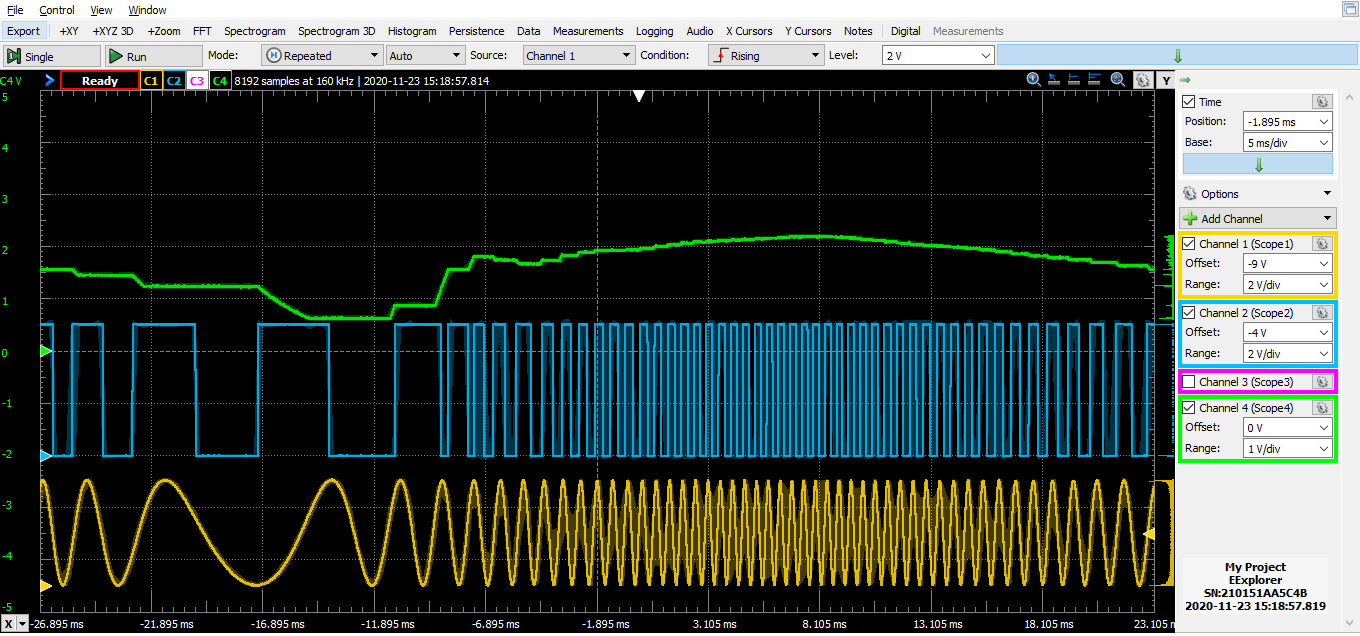
\includegraphics[width= 0.8\textwidth]{../1. PLL/Imagenes/Modulacion090.png}
	\centering
	\caption{Modulación con un índice de $90\%$}
\end{figure}


Variando la frecuencia se puede ver como a $500Hz$ también se pierde la modulación al ser muy baja la frecuencia de la portadora, debiendo así elevar esta frecuencia para poder transmitir el mensaje. Por otro lado superando los 1300Hz se empieza a notar error en la modulación, teniendo así un rango para modular que va entre los $700Hz$ y los $1300Hz$. A continuación se pueden ver las mediciones.

\begin{figure}[H]
	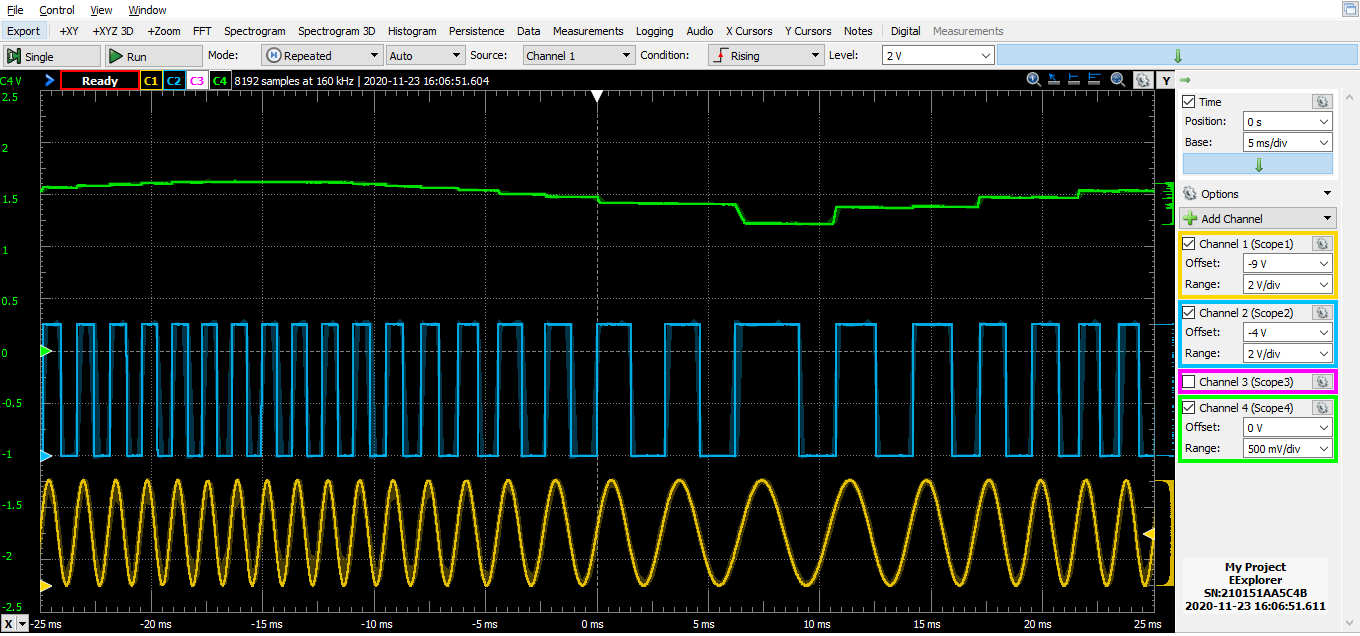
\includegraphics[width= 0.8\textwidth]{../1. PLL/Imagenes/ModFrec500.png}
	\centering
	\caption{Modulación con $f_c=500Hz$}
\end{figure}


\begin{figure}[H]
	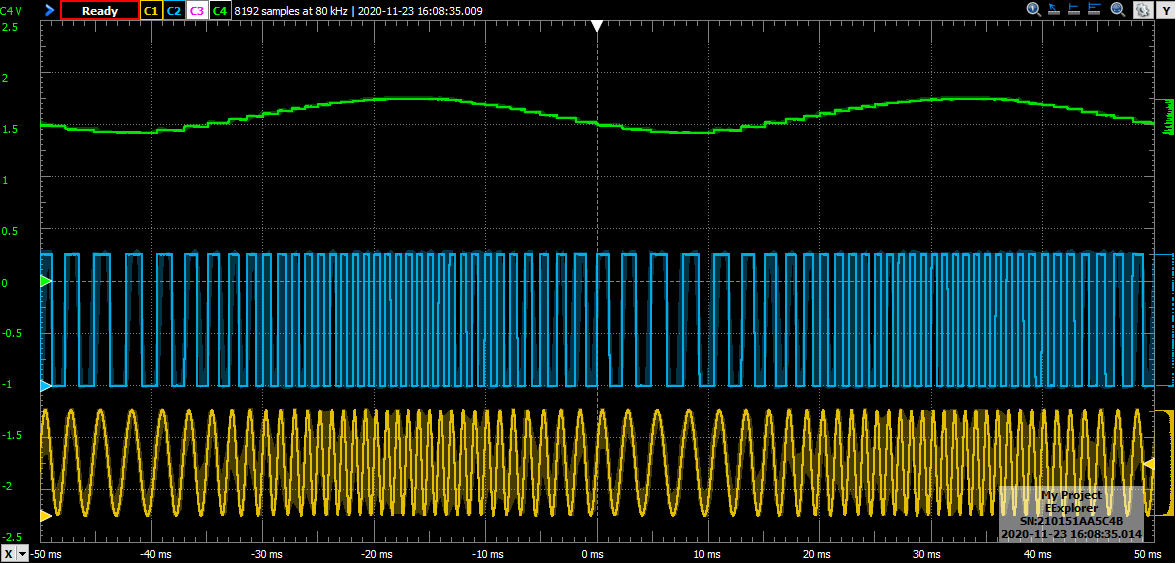
\includegraphics[width= 0.8\textwidth]{../1. PLL/Imagenes/ModFrec700.png}
	\centering
	\caption{Modulación con $f_c=700Hz$}
\end{figure}

\begin{figure}[H]
	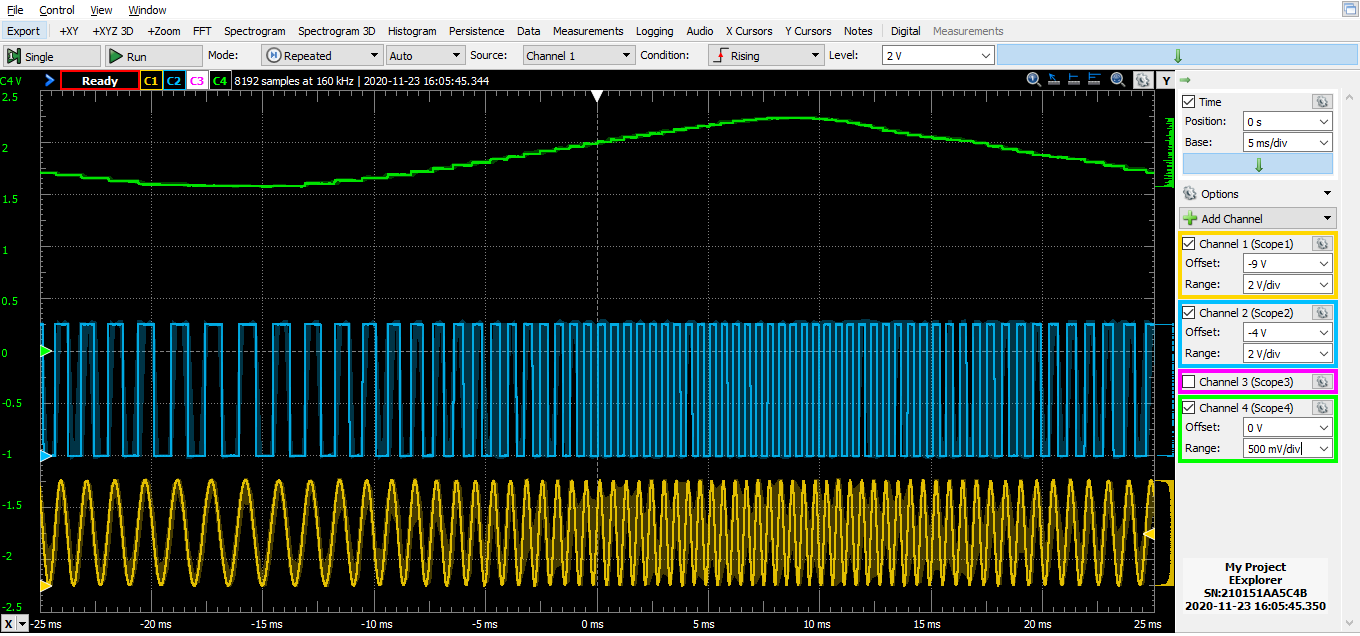
\includegraphics[width= 0.8\textwidth]{../1. PLL/Imagenes/ModFrec1300.png}
	\centering
	\caption{Modulación con $f_c=1300Hz$}
\end{figure}

\begin{figure}[H]
	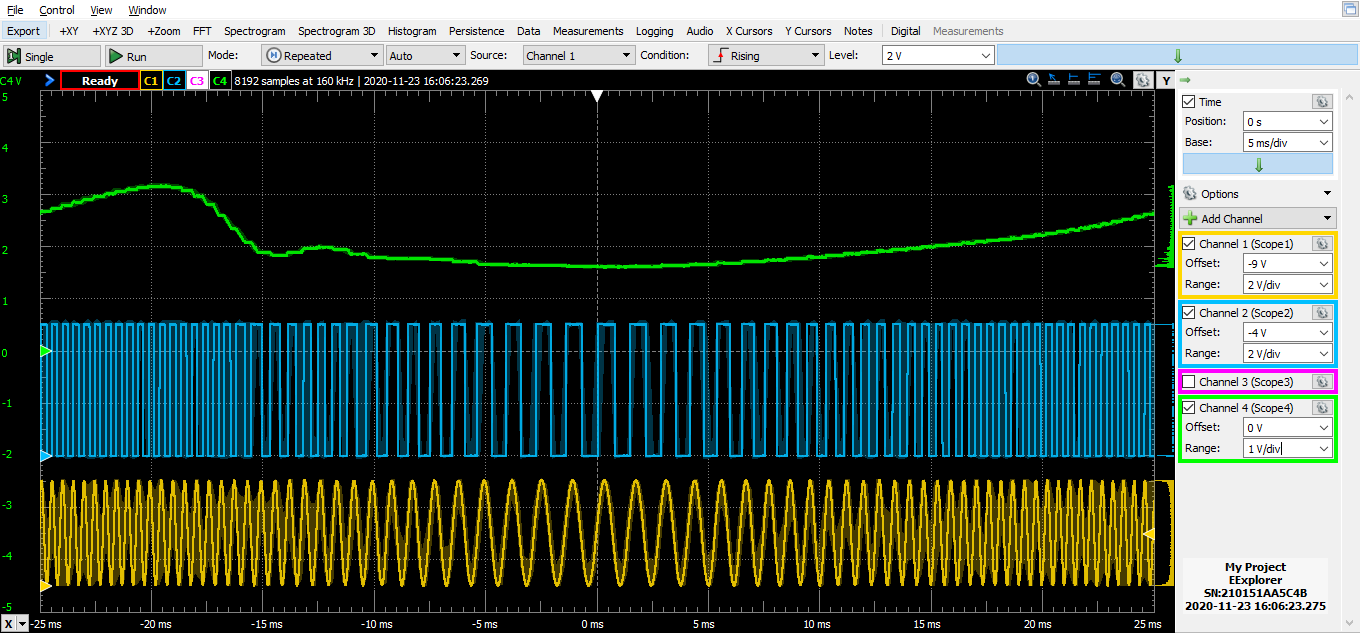
\includegraphics[width= 0.8\textwidth]{../1. PLL/Imagenes/ModFrec1400.png}
	\centering
	\caption{Modulación con $f_c=1400Hz$}
\end{figure}

Cabe destacar que la modulación en FM necesita por lo tanto tener una frecuencia aceptable, un índice de modulación que este entre el $30\%$ y $70\%$, y un valor de tensión de $3V_{pp}$ sin que esta señal llegue a ser negativa. Si no se cumplen estas condiciones el PLL no podrá modular la señal de mensaje o directamente no enganchara la señal de entrada.


\subsection{Respuesta al escalón}
Se ingresó un escalón en frecuencia para poder observar la respuesta transitoria que genera el PLL. Para esto se volvió a usar la opción de \textit{modulation} pero en vez de que la señal de mensaje fuera una sinusoidal se cambio por un pulso. Luego se fue variando el índice de modulación hasta poder obtener una medición fácil de leer esperando una respuesta subamortiguada.
En la medición tomada (figura \ref{fig:REspEscalon}) se puede observar que la señal tarda 12ms en establecerse la señal, un tiempo muy corto ya que estamos usando un filtro RRC, de haber usado un filtro RC hubieramos visto un tiempo mas prolongado.

\begin{figure}[H]
	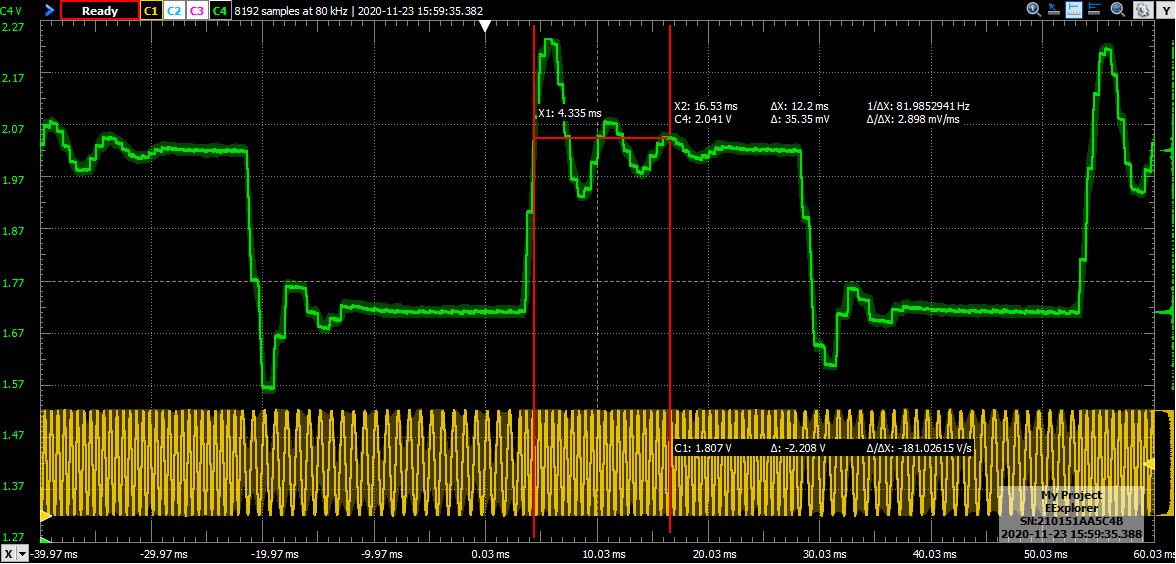
\includegraphics[width= 0.8\textwidth]{../1. PLL/Imagenes/RespEscalonMedicion.png}
	\centering
	\caption{Respuesta al escalón}
	\label{fig:REspEscalon}
\end{figure}

\subsection{Multiplicador de frecuencia}
Dado que el PLL engancha la frecuencia que tiene a la entrada del comparador con la frecuencia de la señal de entrada, que es la otra entrada del comparador, si se coloca un divisor de frecuencia por N a la salida del VCO, se tiene que:

\begin{equation}
	f_{VCO} = N . f_{comp} = N . f_{in}
\end{equation}

Por lo tanto, con un divisor de frecuencia se obtiene un multiplicador de frecuencia. En la implementación se uso el CD4017 para dividir la frecuencia del VCO. Para ello se conecto a la salida del VCO la entrada del clock del divisor(pin 14), y se utilizo como salida el pin 2, el cual corresponde al menor divisor de frecuencia que tiene el integrado, para poder empezar a medir, además de colocar los pines correspondientes tanto a tierra como a alimentación, se debe conectar el pin de reset al pin por el cual quiero dividir mi frecuencia siendo así que esta conexión determina por cuanto se multiplica la frecuencia de mi entrada. 

\begin{figure}[H]
	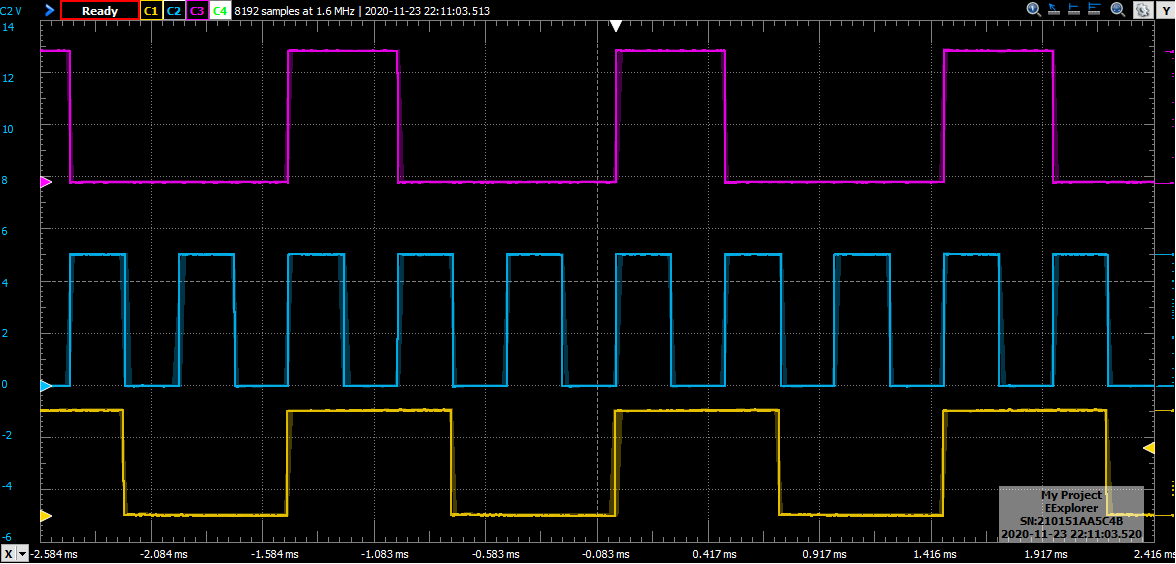
\includegraphics[width= 0.8\textwidth]{../1. PLL/Imagenes/DIV3f680.png}
	\centering
	\caption{Divisor de frecuencia ($N=3$ , $f=680Hz)$}
	\label{fig:Div3Frec680}
\end{figure}

Como se puede apreciar en la figura \ref{fig:Div3Frec680} se utilizo el reset conectado para dividir la frecuencia del VCO en 3. Pero esto tiene limitaciones ya que al cambiar la frecuencia con la que se compara la señal de entrada genera que el enganche del sistema sea alterado, al haber multiplicado la frecuencia de entrada se divide la frecuencia por la cual se puede enganchar, por ende el enganche ha sido reducido por 3. Como se puede ver en la figura \ref{fig:Div3Frec700} al usar una frecuencia mayor al nuevo rango de enganche se pierde este efecto sobre el sistema generando una señal corrida no estable.


\begin{figure}[H]
	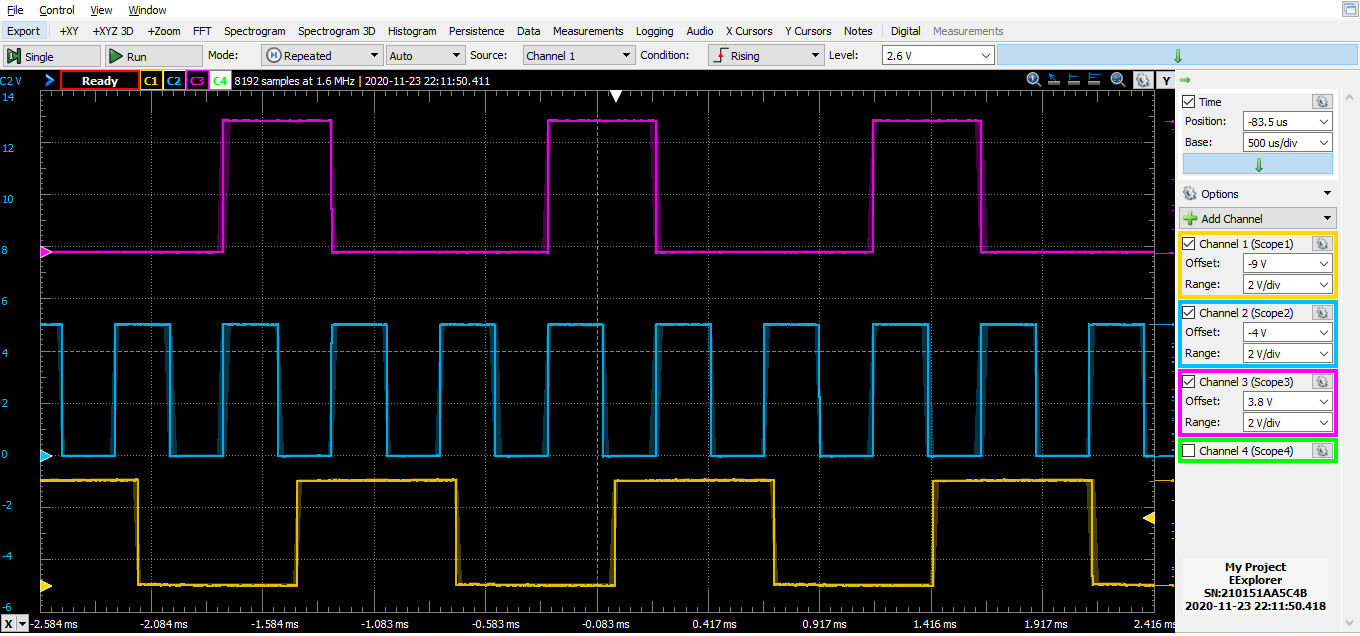
\includegraphics[width= 0.8\textwidth]{../1. PLL/Imagenes/DIV3f700.png}
	\centering
	\caption{Divisor de frecuencia ($N=3$ , $f=700Hz)$}
	\label{fig:Div3Frec700}
\end{figure}

Por otro lado, el valor mínimo no es el establecido en un principio divido N, sino que el filtro no permite que el valor sea menor, sino incluso mayor. Al haber dividido con $N=3$ se obtiene un valor mínimo de $350Hz$ para establecer el enganche. Este valor no es directo del divisor. A continuación se puede ver como a $300Hz$ se pierde el enganche:

\begin{figure}[H]
	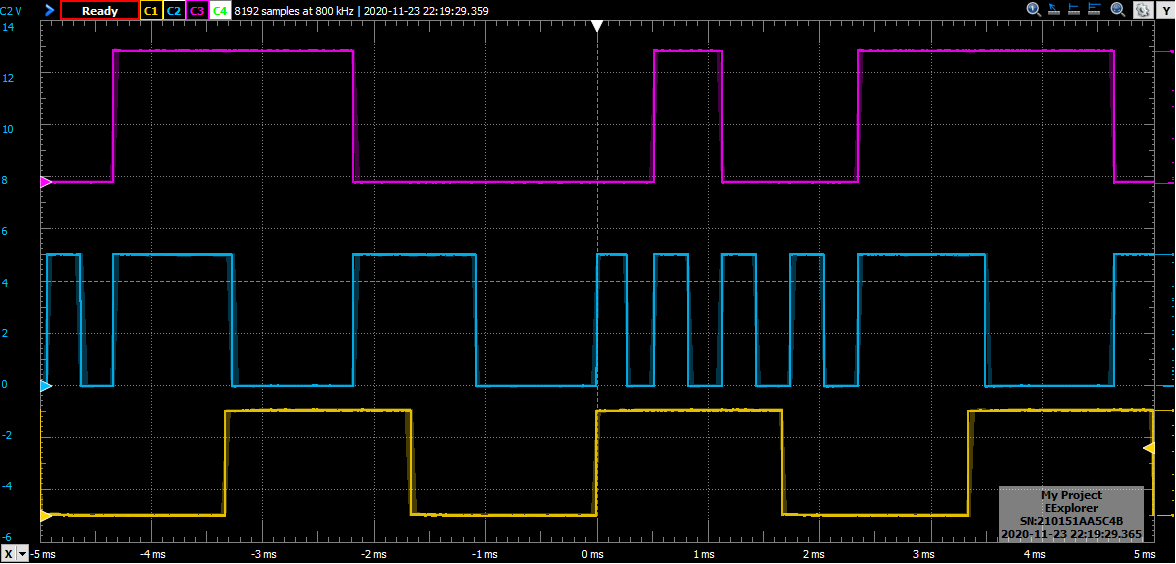
\includegraphics[width= 0.8\textwidth]{../1. PLL/Imagenes/DIV3f300.png}
	\centering
	\caption{Divisor de frecuencia ($N=3$ , $f=300Hz)$}
	\label{fig:Div3Frec300}
\end{figure}

Por último se comprobó que no es posible dividir por cualquier cantidad ya que al usar un N muy grande se pierde el rango de enganche, haciendo que el sistema se vuelva inútil, por lo cual a la hora de dividir la frecuencia del VCO se debe tener en cuenta hasta que valor puede llegar a dividirse. En la figura \ref{fig:Div8Frec250} se puede ver que usando un valor de $N=8$ y una frecuencia de $250Hz$ se obtiene un buen enganche, pero con un rango muy acotado. Utilizando un $N=10$ no se logró encontrar un valor de enganche.

\begin{figure}[H]
	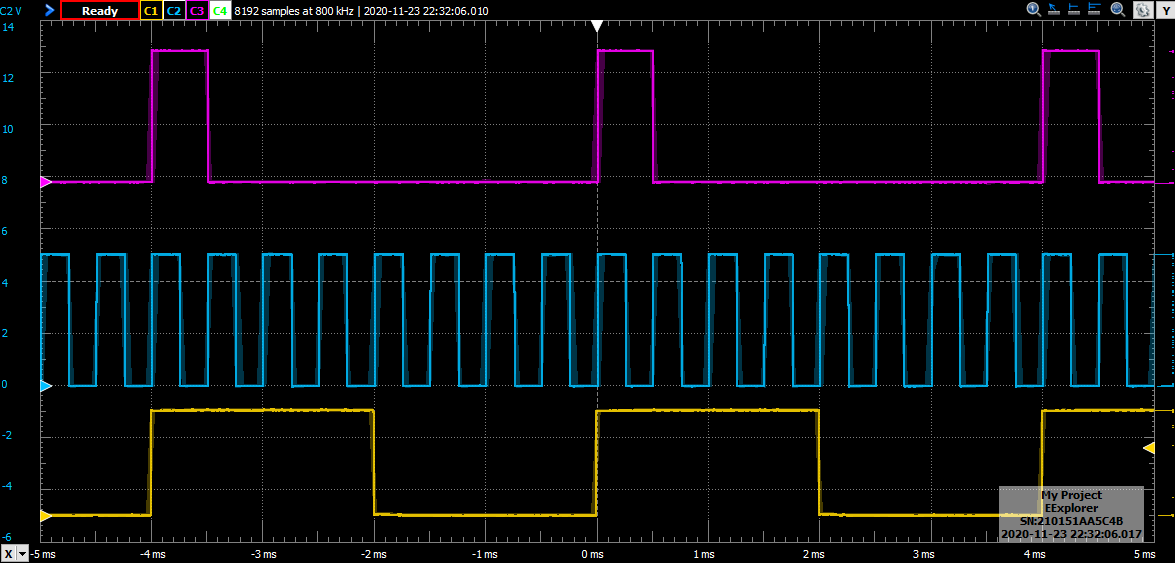
\includegraphics[width= 0.8\textwidth]{../1. PLL/Imagenes/DIV8f250.png}
	\centering
	\caption{Divisor de frecuencia ($N=8$ , $f=250Hz)$}
	\label{fig:Div8Frec250}
\end{figure}

\subsection{Conclusión}
Se pudo ver las diferentes utilidades del PLL y como puede usarse tanto para modulación como para multiplicar la frecuencia de entrada. Se pudo demostrar que no es posible ambos usos con cualquier parámetro, sino que se deben cuidar los rangos donde se pueden utilizar ambos modos de uso. 
\newline
En el caso del uso de modulación FM se pudo ver como afecta el indice de modulación a la señal de mensaje y que errores existen en la modulación cuando no se trabaja con un correcto valor de trabajo.
\newline
En el caso del multiplicador de frecuencia se pudo notar las complicaciones que tiene usar un divisor muy alto en el VCO, dejando sin enganche al sistema. 



\end{document}